\documentclass[12pt, a4paper]{article}
\usepackage{amsmath}
\usepackage{amsfonts}
\usepackage{amsthm}
\usepackage{mathtools}
\usepackage{tikz}
\usetikzlibrary{bayesnet}
\newtheorem{theorem}{Theorem}[section]
\newtheorem{definition}{Definition}[section]
\numberwithin{equation}{section}
\usepackage{pgfplots}
\pgfplotsset{width=10cm,compat=1.9}
\graphicspath{ {img/} }
\DeclareGraphicsExtensions{.png}

\title{Process Mining}
\author{Kristian Wichmann}

\begin{document}
\maketitle

\section{Event logs}
An \textit{event log} is a collection of data where each row contains at least the following:
\begin{itemize}
\item A \textit{case id} corresponding to a particular unit whose processes we wish to discover.
\item An \textit{event id}, to denote a specific kind of activity.
\item A \textit{timestamp}, which allows us to order the events.
\end{itemize}

\section{Model: Petri nets}

\subsection{Petri net graphs}
A \textit{Petri net graph} is a tuple $(P, T, F)$. Here $P$ is a collection of \textit{places} and $T$ a collection of \textit{transitions}, $P$ and $T$ disjoint. The \textit{flow relations} $F\subseteq(P\times T)\cup(T\times P)$ corresponds to place inputs ($I\subseteq P\times T$) and outputs ($O\subseteq T\times P$) to transitions.

\begin{figure}
\centering
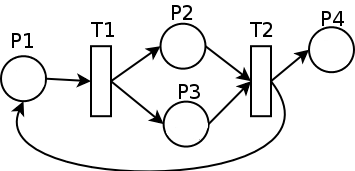
\includegraphics[width=0.7\textwidth]{petri_graph}
\caption{An example of a Petri net graph.}
\label{fig:petri_graph}
\end{figure}

The graphical representation of a petri net graph is to draw places as circles, transitions as thick lines or squares, and flow relations as arrows from places to transitions. As an example, figure \ref{fig:petri_graph} is the graphical representation of the following Petri net graph:
\begin{itemize}
\item $P=\{P1, P2, P3, P4\}$
\item $T=\{T_1, T_2\}$
\item $F=I\cup O$, where:
\begin{align}
I=&\{\{P1, T1\}, \{P2, T2\}, \{P3, T2\}\}\\
O=&\{\{T1, P2\}, \{T1, P3\}, \{T2, P1\}, \{T2, P4\}\}
\end{align}
\end{itemize}

Sometimes, we may wish to allow more than one arrow between a place-transition/transition-place pair. In this case, $F$ instead becomes a function:
\begin{equation}
F: (P\times T)\cup(T\times P)\rightarrow\mathbb{N}_0
\end{equation}
The value of a pair is then the number of arrows. Again, this could be split into input and output functions:
\begin{equation}
I: P\times T\rightarrow\mathbb{N}_0,\quad
O: T\times P\rightarrow\mathbb{N}_0
\end{equation}

\subsection{Markings and Petri nets}

\begin{figure}
\centering
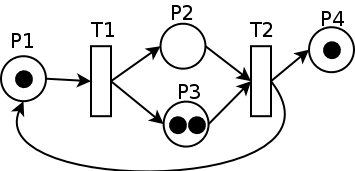
\includegraphics[width=0.7\textwidth]{petri_marking}
\caption{An example of a Petri net.}
\label{fig:petri_marking}
\end{figure}

A \textit{marking} $M$ on a Petri net graph, is a function:
\begin{equation}
M: P\rightarrow\mathbb{N}_0
\end{equation}
This is interpreted as the number of \textit{tokens} present at each place in the Petri net graph. For instance, figure \ref{fig:petri_marking} shows the following marking on the example Petri net graph from the section above:
\begin{equation}
P1\mapsto 1,\quad P2\mapsto 0,\quad P3\mapsto 2,\quad P4\mapsto 1
\end{equation}

A collection of a Petri net graph $(P, T, F)$ and an initial marking $M_0$ on it is called a \textit{Petri net}.

\subsection{Rules of the "game"}
From the initial marking, a Petri net can undergo the transitions in $T$ under certain circumstances.

A transition $t\in T$ is \textit{enabled}, if all the places which has an input flow relation pointing to it all has at least one token\footnote{If several arrows are allowed, each place has to hold at least a number of tokens corresponding to the number or arrows.}.

An enabled transition may \textit{fire}, which means that the current marking changes, such that each token from the input places are removed, while all the output places gets a token\footnote{Again, if several arrows are allowed, several tokens are removed/added according to the multiplicity of arrows.}.

Transitions always happens in a specific order, so two transitions cannot fire at the same time. This means that we may write a \textit{trajectory} of the Petri net as:
\begin{equation}
M_0, M_1, M_2, \ldots,\quad \langle t_1,t_2,\cdots\rangle
\end{equation}
Here, all the $M_i$'s are markings, and between $M_i$ and $M_{i+1}$ transition $t_{i+1}$ fires. Such a trajectory may or may not be finite in length.

The set of all markings that are \textit{reachable} for a Petri net $N$ is denoted $R(N)$. The elements of $R(N)$ forms a directed \textit{reachability graph}, with transitions as edges.

\subsection{Properties of Petri nets}
A marking where no transitions are enable is called \textit{deadlocked}. A Petri net with a deadlocked marking in its reachability graph is said to have a \textit{potential deadlock}.

A transition in a Petri net that can never fire, i.e. is not an edge anywhere in the reachability graph is called \textit{dead} or $L_0$-\textit{live} (a designation that will become clear in a while). A transition that is not dead has some degree of being alive, as shown below:
\begin{itemize}
\item A transition is $L_1$-\textit{live} if it is not dead, i.e. if is occurs as an edge somewhere in the reachability graph. This is also called \textbf{potentially fireable}.
\item  A transition is $L_2$-\textit{live} if for any positive integer $k$ there is a reachable marking in which it occurs at least $k$ times on a trajectory to the marking. (The trajectories can be different for each $k$).
\item  A transition is $L_3$-\textit{live} if there is a trajectory in which the transition occurs infinitely often.
\item  A transition is $L_4$-\textit{live} - or simply \textit{live}, if for any reachable marking, the transition is $L_1$-live. I.e. no matter where in the reachability graph we are, it is always possible to fire the transition some time in the future.
\end{itemize}
These conditions are progressively stronger, so usually only the highest index is used to refer to a given transition.

A place $p$ in a Petri net is called $k$-\textit{bounded} if all markings in the reachability graph has as most $k$ tokens on it. A place that is 1-bounded is called \textit{safe}. A place that is $k$-bounded for any positive value of $k$ is called \textit{bounded}.

A Petri net in which all places are ($k$-)bounded is called  ($k$-)\textit{bounded}. A Petri net in which all places are safe is called \textit{safe}. A Petri net graph in which all possible initial markings are bounded is called \textit{structurally bounded}.

\subsection{Workflow nets}
A \textit{workflow net} (or WF net for short) is a Petri net which has a start or \textit{source} place and an ending or \textit{sink} place, so that the source has no inputs, and the sink no outputs. It is used to model processes with transitions representing events.

\section{The alpha algorithm}

\section{Model: Dependency graph}
A \textit{dependency graph} is a series of nodes - representing events - in which there are causal arrows between events. So as such, this is simply a directed graph. 

\section{Heuristics mining}

\end{document}